% !TeX spellcheck = de_DE
\section{\ExercisePrefixMemory Debugging \optional}\label{sec:debugging}
\optionaltextbox

Die meisten Entwicklungsgebungen bieten Debuggingfunktionalität.
Debugging ermöglicht es schrittweise die Ausführung des Codes zu beobachten und lokale Variablen zu inspizieren und auf ihren aktuellen Wert zu prüfen. Oftmals ist diese Vorgehensweise gut geeignet kleinere Fehler in der Programmlogik zu finden.
Dazu kann man Breakpoints festlegen, an denen die Ausführung des Programms anhält.

Wir arbeiten in dieser Aufgabe mit einer absichtlich fehlerhaften Implementierung der einfachverketteten Liste (siehe \ref{sec:linkedList}).
Importiere dazu das Projekt unter folgendem Pfad: \cpppLinkToSampleSolution{debug_linked_lists}{debug\_linked\_lists}.

Diese setzt du in CodeLite mit einem Linksklick der Zeile in welcher der Ablauf stoppen soll wie in den Zeilen~8 und~12 in \Cref{fig:breakpoints}. 
Nutze für diese Aufgabe die Vorlage für das Debugging von \ref{sec:linked_list}. Starte den Debugger über \menuPath{Debugger \menuSep Start/Continue Debugger}.
Du wirst sehen, dass die Ausführung in Zeile 8 stoppt, was durch den grünen Pfeil markiert wird. 
Mit einem Klick auf den Continue-Button 
\includegraphics[height=1.5ex]{02_memory/figures/continueButton.png} lässt sich der Programmablauf fortsetzen.
Mit dem Next-Button  
\includegraphics[height=1.5ex]{02_memory/figures/stepOverButton.png} wird die aktuelle Zeile ausgeführt und der Programmzeiger springt in die nächste Zeile.
Der Step-In-Button 
\includegraphics[height=1.5ex]{02_memory/figures/stepInButton.png} bewirkt, dass in die erste Zeile der aufgerufenen Funktion gesprungen wird.
Der Step-Out-Button  
\includegraphics[height=1.5ex]{02_memory/figures/stepOutButton.png} führt den Code bis zum \lstinline|return|-Statement aus und springt zurück und setzt den Programmzeiger hinter die aufgerufene Funktion.
Im Fenster rechts unten (\Cref{fig:locals_view}) kannst du die Werte der Variablen inspizieren und solltest sehen, dass \lstinline|current_size| beim ersten Breakpoint den Wert 2 besitzt.
Gegebenenfalls musst du die Ansicht mithilfe der blauen Schaltfläche 
\includegraphics[height=1.5ex]{02_memory/figures/updateLocalsButton.png} aktualisieren.
Zudem kannst du während dem Debugging über einen Rechtsklick auf eine Zeile und den Menüeintrag \enquote{Run to here} den Code bis zu dieser Zeile ausführen.
 
%Beispiel: linked list != Operator fehler einbauen und finden lassen. dabei vorgeben wo Breakpoint gesetzt werden soll und dann inspizieren lassen...
 
Setze nun in Zeile 25 von \lstinline{main.cpp} einen Breakpoint und versuche mit Hilfe des Debuggers herauszufinden, warum die Liste nicht ausgegeben wird.
%
\begin{figure}
	\centering
	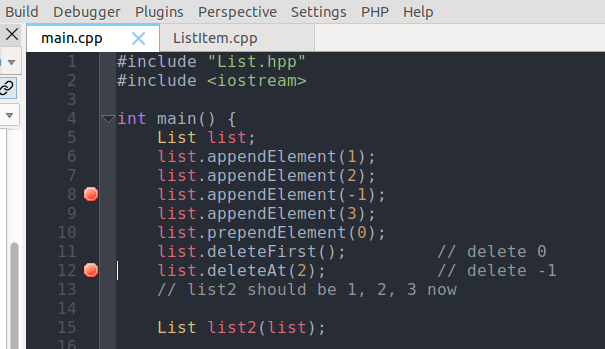
\includegraphics[width=.6\textwidth]{02_memory/figures/breakpoints.png}
	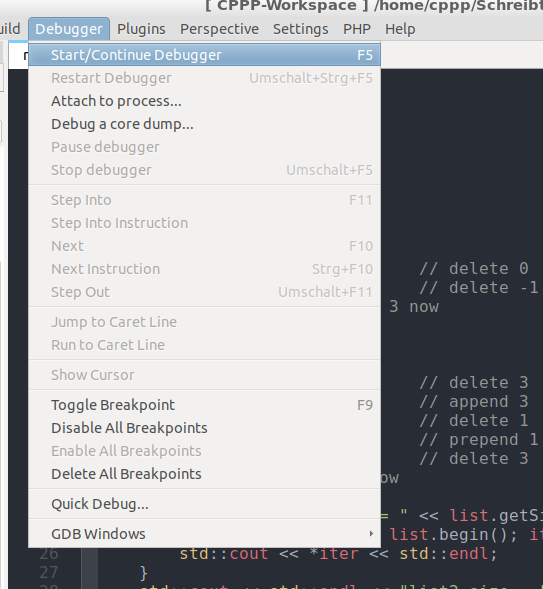
\includegraphics[width=.3\textwidth]{02_memory/figures/start_debugger.png}
	\caption{Setze Breackpoints und starte Debugger}
	\label{fig:breakpoints}
\end{figure}

%\begin{figure}
%	\centering
%	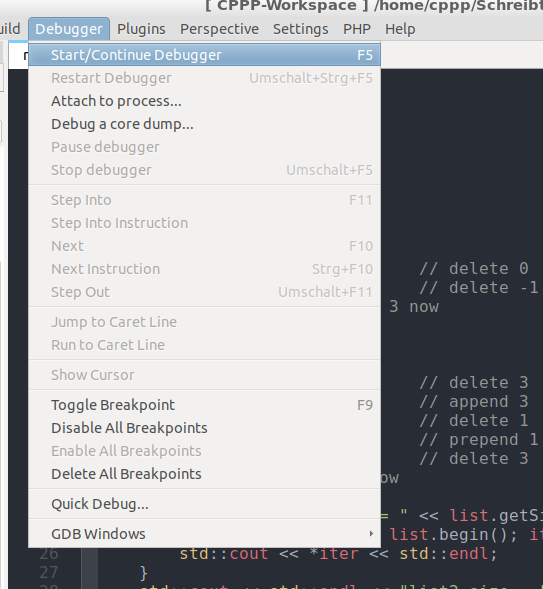
\includegraphics[width=.9\textwidth]{02_memory/figures/start_debugger.png}
%	\caption{Starte den Debugger}
%	\label{fig:start_debugger}
%\end{figure}

\begin{figure}
	\centering
	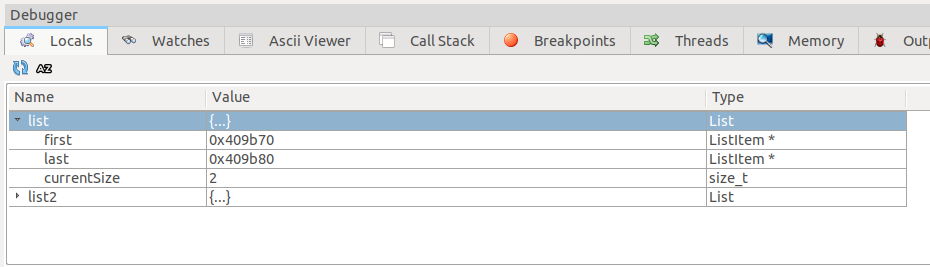
\includegraphics[width=.9\textwidth]{02_memory/figures/locals_view.png}
	\caption{Inspizieren von Variablen}
	\label{fig:locals_view}
\end{figure}

%\begin{figure}
%	\centering
%	
\includegraphics[width=.9\textwidth]{02_memory/figures/debugtools.png}
%	\caption{Debug Werkzeuge: }
%	\label{fig:debug_tools}
%\end{figure}

\hints{
	\item Mit dem Step-In-Button  
\includegraphics[height=1.5ex]{02_memory/figures/stepInButton.png} kannst du auch die Aufrufe sehen, welche im \lstinline|for|-Schleifenkopf gemacht werden.
    \item Überprüfe die Rückgabe von \lstinline|operator!=|.
}